\section{Diode Circuits II}

\subsection{Experiment Design}
    \subsubsection{Background}
    In this experiment, we want to verify the half-wave rectifier, clipper, and clamper circuits.

    \subsubsection{Propose}
    \begin{itemize}
        \item To verify a half-wave diode rectifier circuit
        \item To verify clipper circuits and clamper circuits
    \end{itemize}

\subsection{Experiment Design}
    \subsubsection{Materials}
        In this experiment, we will use the following components:
        \begin{itemize}
            \item 1N4148 Diode
            \item Resistors
            \item Breadboard
            \item Signal Generator
            \item DC Power Supply
            \item Digital Multimeter
            \item Oscilloscope
        \end{itemize}

    \subsubsection{Circuit Diagram}
        The following circuit diagrams 
        \begin{figure}[H]
            \centering
            \begin{subfigure}{0.4\textwidth}
                \includegraphics[width=1\linewidth]{Experiment_02/Circuits/Lab2a.png}
                \caption{Half-wave rectifier}
                \label{cir:2a}
            \end{subfigure}
            \begin{subfigure}{0.4\textwidth}
                \includegraphics[width=1\linewidth]{Experiment_02/Circuits/Lab2b.png}
                \caption{Clipper circuit}
                \label{cir:2b}
            \end{subfigure}

            \begin{subfigure}{0.4\textwidth}
                \includegraphics[width=1\linewidth]{Experiment_02/Circuits/Lab2c.png}
                \caption{Clipper circuit IIII}
                \label{cir:2c}
            \end{subfigure}
            \begin{subfigure}{0.4\textwidth}
                \includegraphics[width=1\linewidth]{Experiment_02/Circuits/Lab2d.png}
                \caption{Clamper circuit}
                \label{cir:2d}
            \end{subfigure}

            \caption{The circuit diagrams}
        \end{figure}

    \subsubsection{Theoretical Analysis}
        \begin{enumerate}[a]
            \item \textbf{Half-wave Rectifier}\par
                From the circuit diagram \ref{cir:2a}. One may easily write the output voltage with respect to the input voltage as follows:
                \begin{equation}
                    \begin{cases}
                        V_o = V_s - V_\gamma & V_s \ge V_\gamma\\
                        V_o = 0 & V_s < V_\gamma\\
                    \end{cases}
                \label{eq:2ret}
                \end{equation}
                where $V_s$ is the input voltage, $V_o$ is the output voltage, and $V_\gamma$ is the diode build in voltage.
            
            \item \textbf{Clipper Circuit}\par
                The clipper circuit is a circuit that clips the input voltage to a certain level. According to \ref{cir:2b} The output voltage can be written as follows:
                \begin{equation}
                    \begin{cases}
                        V_o = V_\gamma + V_s & V_B - V_\gamma \ge V_s\\
                        V_o = V_B & V_s > V_B - V_\gamma\\
                    \end{cases}
                \label{eq:2clip}
                \end{equation}
                where $V_s$ is the input voltage, $V_B$ is a DC power supply, $V_o$ is the output voltage, and $V_\gamma$ is the diode build in voltage.
            
            \item \textbf{Clipper Circuit II}\par
                The clipper circuit shown in figure \ref{cir:2c} is a circuit that clips with two limit. And the output voltage have the following expression:
                \begin{equation}
                    \begin{cases}
                        V_o = V_{B_2} & V_s > V_{B_2} - V_\gamma,~\text{Both diodes off}\\
                        V_o = V_{B_2} - R_2(\frac{V_{B_2}-V_\gamma-V_s}{R_1+R_2}) & V_\gamma \le V_s \le V_{B_2} - V_\gamma,~\text{$D_1$ on only}\\
                        V_o = V_\gamma & V_\gamma > V_s,~\text{Both diodes on}\\
                    \end{cases}
                \label{eq:2clip2}
                \end{equation}
                where $V_s$ is the input voltage, $V_{B1}$ and $V_{B2}$ are DC power supply, $V_o$ is the output voltage, and $V_\gamma$ is the diode build in voltage.
                
            \item \textbf{Clamper Circuit}\par
                Circuit shown in figure \ref{cir:2d} is a clamper circuit. Such circuit will
                The output voltage can be written as follows:
                \begin{equation}
                    \begin{cases}
                        V_o = V_s(sin\omega t-1) & V_s > 0\\
                        V_o = V_s - V_C & V_s < 0\\
                    \end{cases}
                \label{eq:2clam}
                \end{equation}
                where $V_s$ is the input voltage, $V_{B1}$ is a DC power supply, $V_o$ is the output voltage, and $V_\gamma$ is the diode build in voltage.
        \end{enumerate}

\subsection{Experiment record}
    \subsubsection{Half-wave Rectifier}
    \begin{enumerate}[I]
        \item \textbf{Data Recorded}\newline
            The recorded data for the integration operation circuit is shown in the following table \ref{tab:}:
            \begin{table}[h]
                \centering
                \begin{tabular}{l|cccccccc}
                    \hline
                    \toprule
                    Vs   & -3     & -2.8   & -2.6   & -2.4   & -2.2   & -2    & -1.8  & -1.6   \\
                    \midrule
                    Vo   & 0      & 0      & 0      & 0      & 0      & 0     & 0     & 0      \\
                    Theo & 0      & 0      & 0      & 0      & 0      & 0     & 0     & 0      \\
                    \midrule
                    \midrule
                    Vs   & -1.4   & -1.2   & -1     & -0.8   & -0.6   & -0.4  & -0.2  & 0      \\
                    \midrule
                    Vo   & 0      & 0      & 0      & 0      & 0      & 0     & 0     & 0      \\
                    Theo & 0      & 0      & 0      & 0      & 0      & 0     & 0     & 0      \\
                    \midrule
                    \midrule
                    Vs   & 0.2    & 0.4    & 0.6    & 0.8    & 1      & 1.2   & 1.4   & 1.6    \\
                    \midrule
                    Vo   & 0.2m   & 10.48m & 101.3m & 0.2587 & 0.431  & 0.614 & 7993  & 0.9886 \\
                    Theo & 0      & 0      & 0      & 0.2    & 0.4    & 0.6   & 0.8   & 1      \\
                    \midrule
                    \midrule
                    Vs   & 1.8    & 2      & 2.2    & 2.4    & 2.6    & 2.8   & 3     &        \\
                    \midrule
                    Vo   & 1.1758 & 1.3674 & 1.561  & 1.752  & 1.9457 & 2.145 & 2.343 &        \\
                    Theo & 1.2    & 1.4    & 1.6    & 1.8    & 2      & 2.2   & 2.4   &        \\
                    \midrule
                \end{tabular}
                \caption{Recorded Data for half-wave rectifier}
                \label{tab:2ret}
            \end{table}
        And here are the plot of response with respect to the input signal:
        \begin{figure}[H]
            \centering
            \begin{subfigure}{0.45\textwidth}
                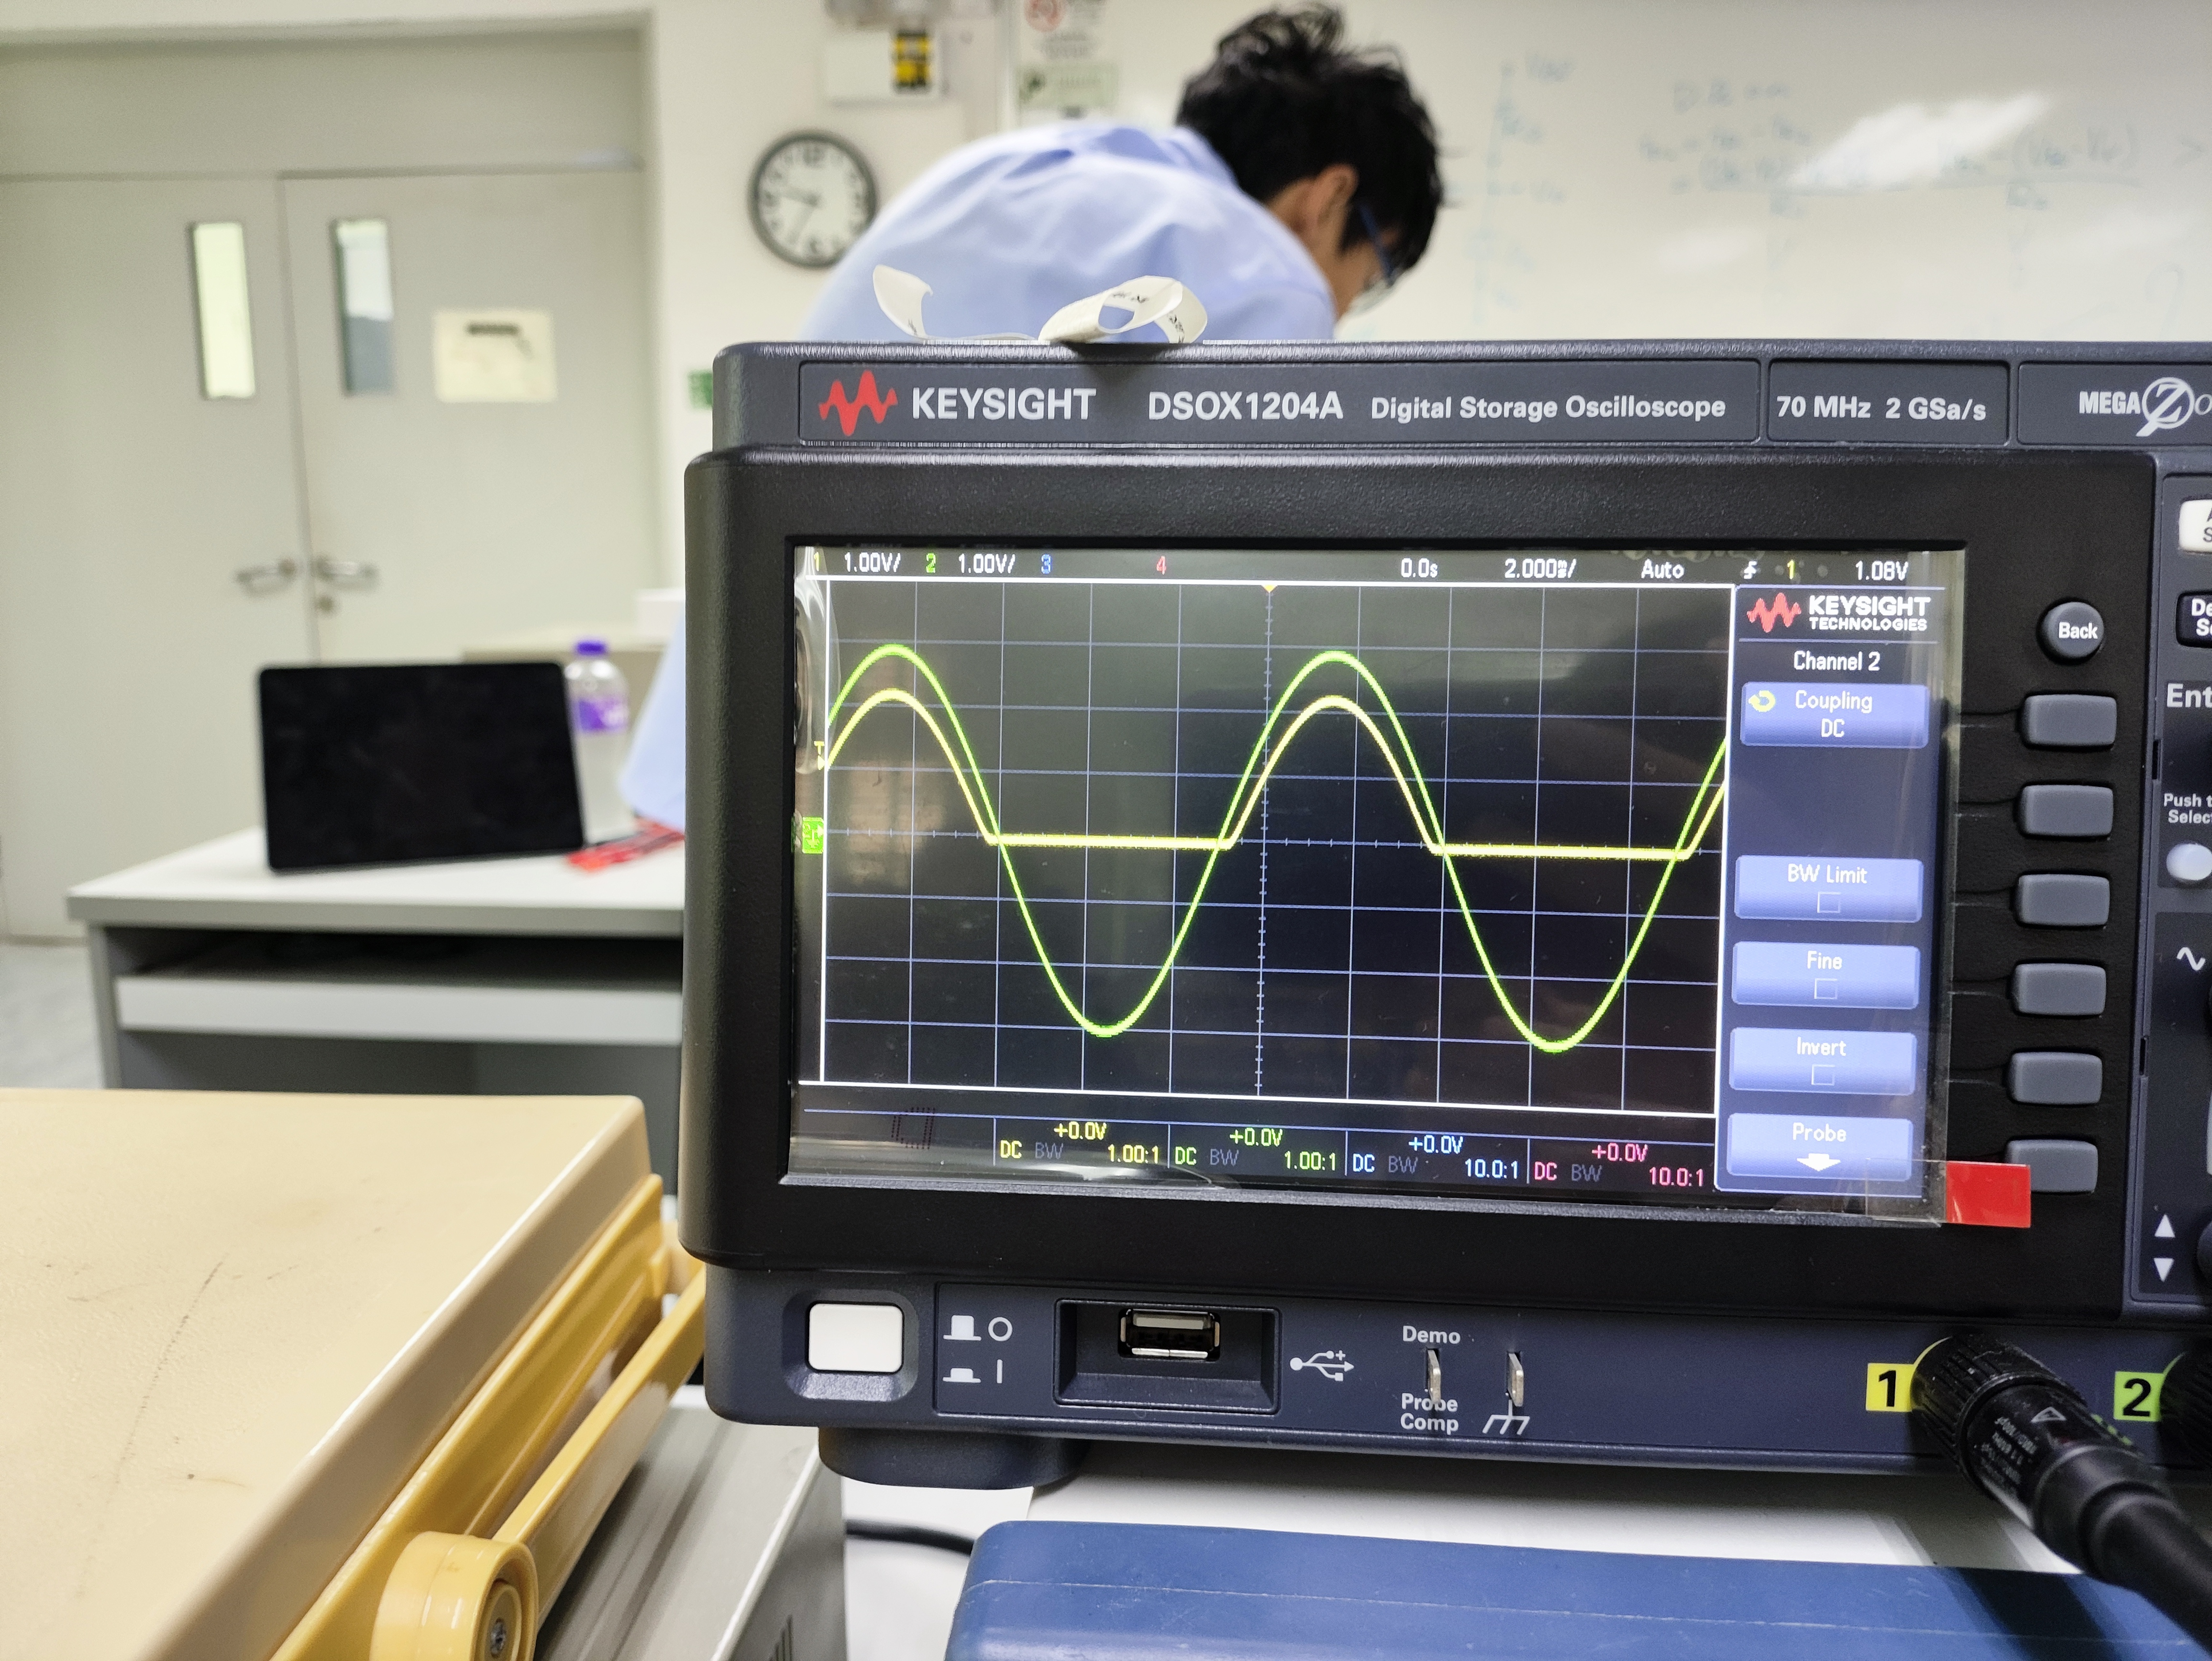
\includegraphics[width=1\linewidth]{Experiment_02/Images/2.4_sin_halfWave.jpg}
                \caption{Sin input signal}
                \label{wave:2aSin}
            \end{subfigure}
            \begin{subfigure}{0.45\textwidth}
                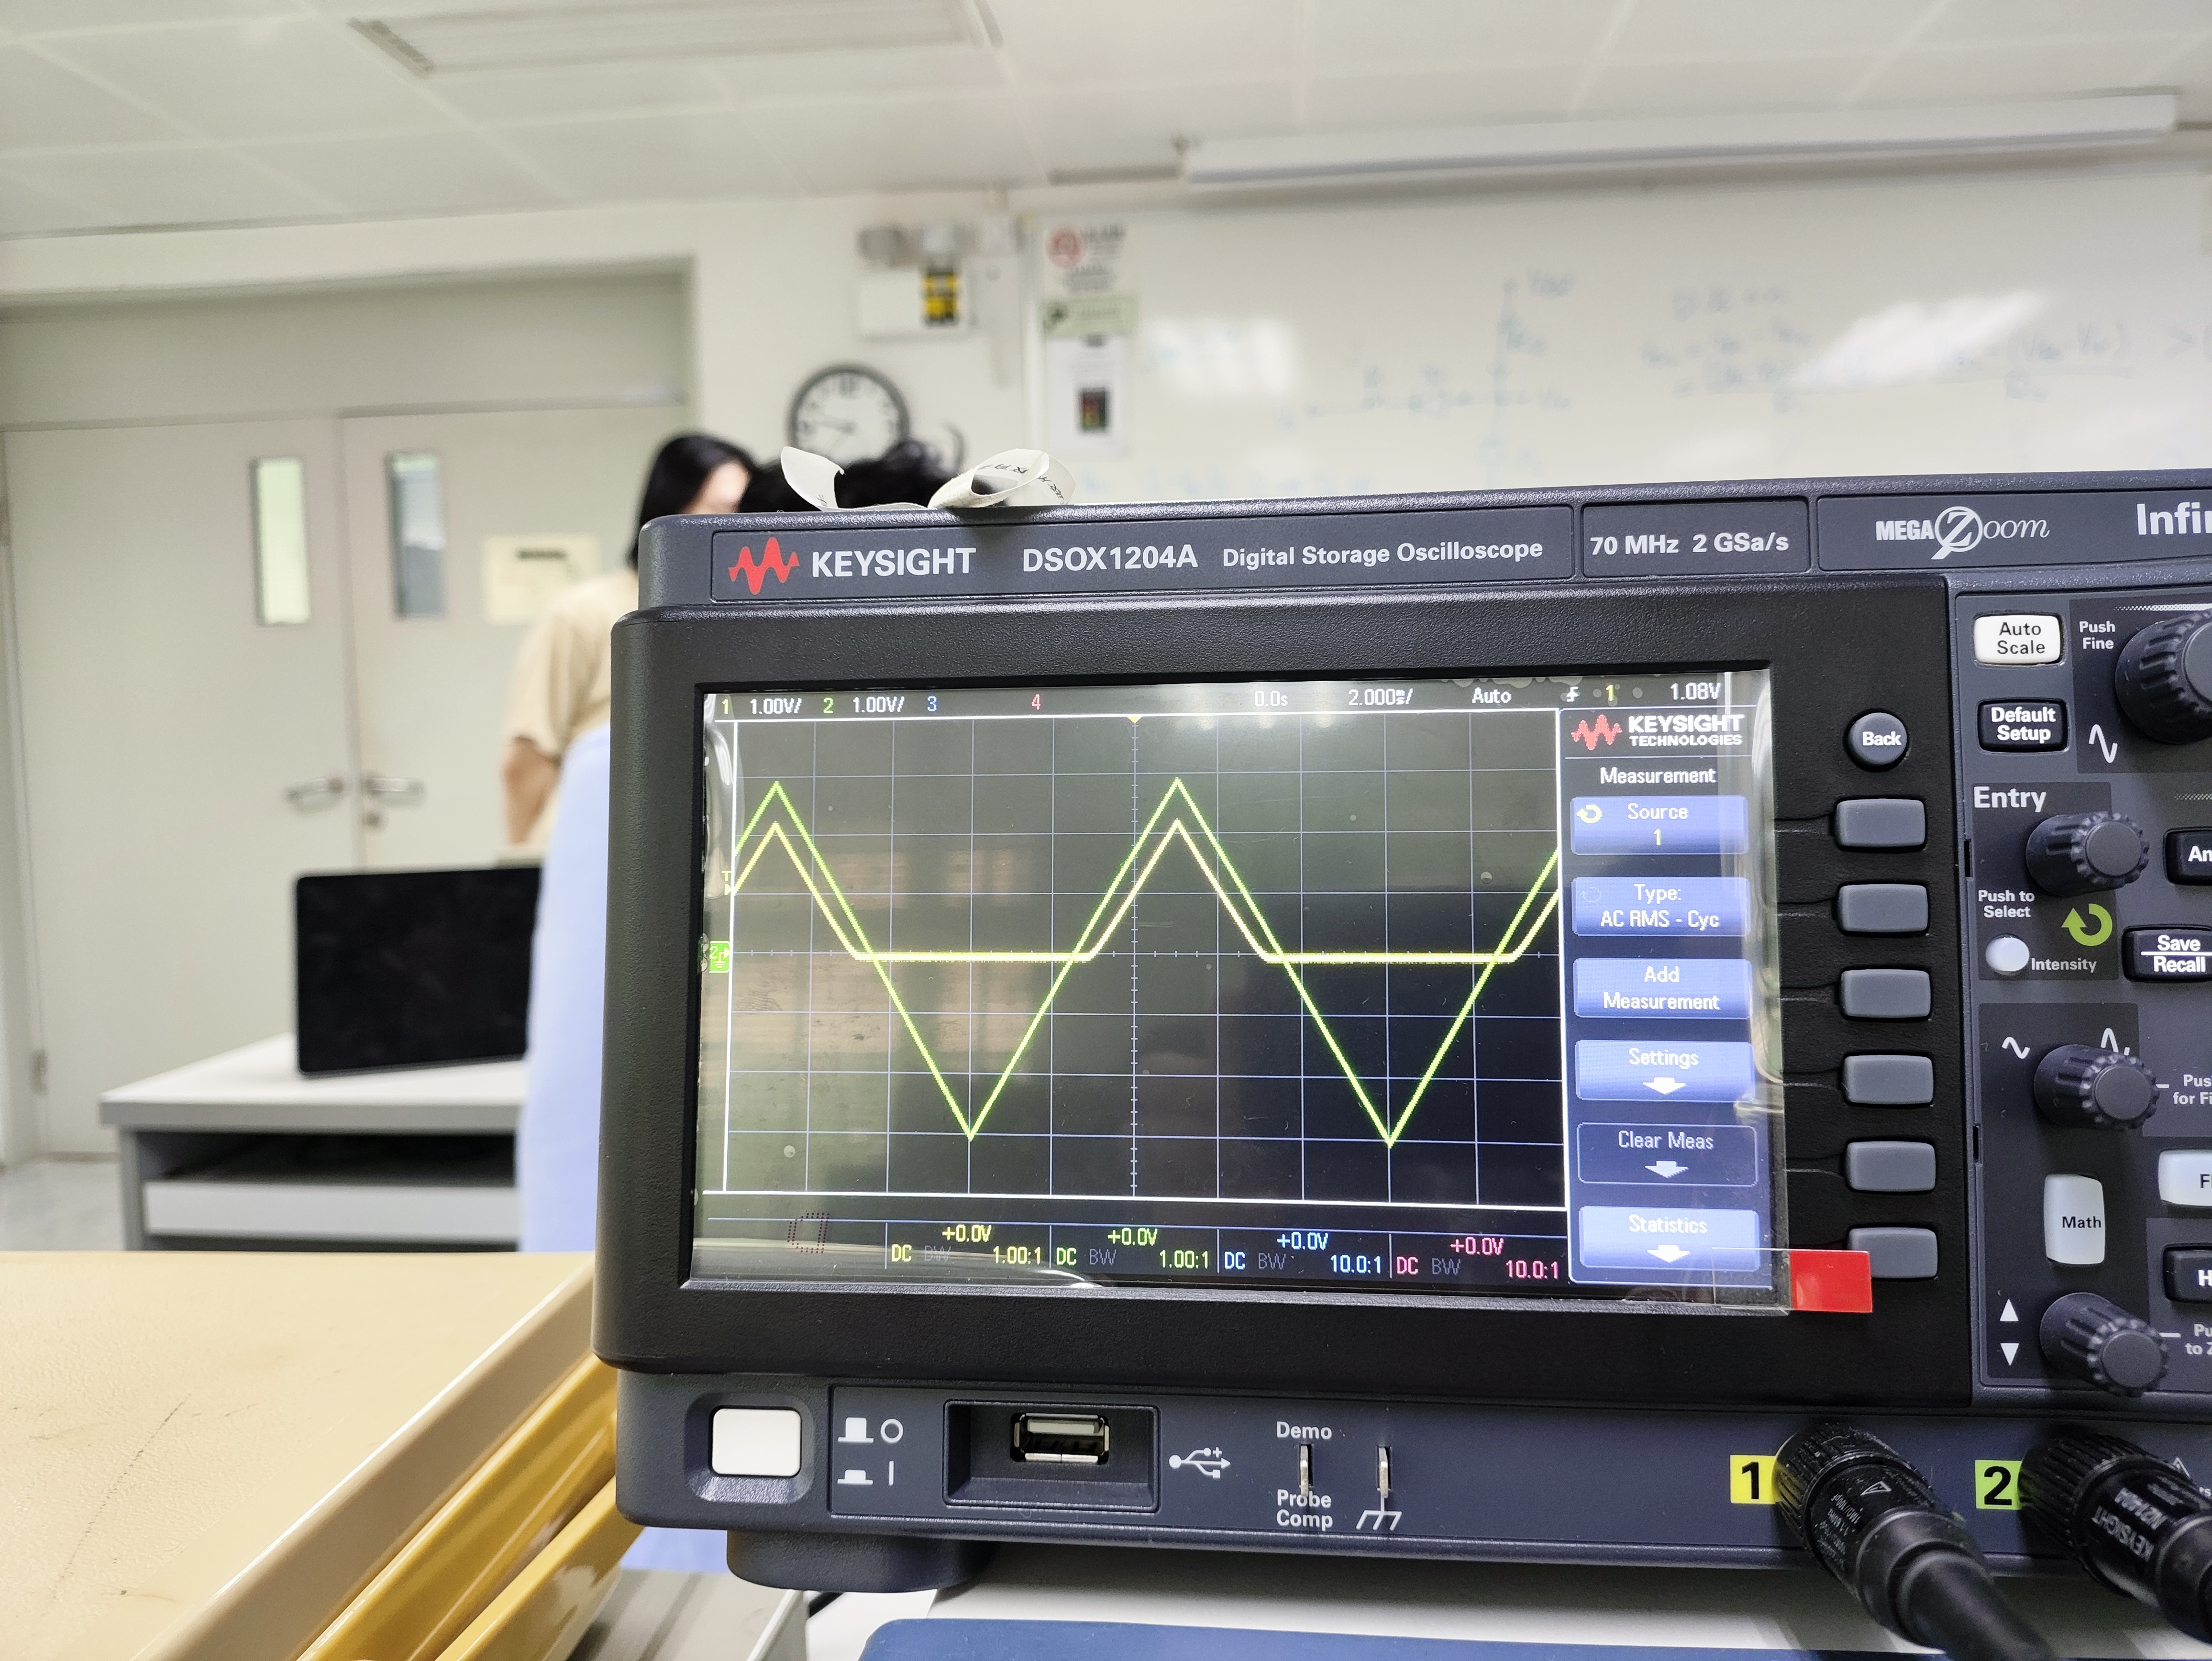
\includegraphics[width=1\linewidth]{Experiment_02/Images/2.4_tri_halfWave.jpg}
                \caption{Triangular input signal}
                \label{wave:2aTri}
            \end{subfigure}
            \caption{The output singal of half-wave rectifier}
        \end{figure}

        \item \textbf{Data Analysis}\newline
            The theoretical output voltage of the half-wave rectifier is caculated according to equation \ref{eq:2ret}, and was put into the table tab\ref{tab:2ret} for reference.\par

            According to the table, the measured output voltage is consistent with the theoretical output voltage. This means the half-wave rectifier works as expected.\par

            In the wavefrom plot in fig\ref{wave:2aSin} and fig\ref{wave:2aTri}, we can see half of the input signal is being clipped by the rectifier, and was reduced by the diode build-in voltage.\par
    \end{enumerate}


    \subsubsection{Clipper Circuit}
    \begin{enumerate}[I]
        \item \textbf{Data Recorded}\newline
            The recorded data for the integration operation circuit is shown in the following table \ref{tab:}:
            \begin{table}[h]
                \centering
                \begin{tabular}{l|cccccccc}
                    \hline
                    \midrule
                    Vs   & -3     & -2.8   & -2.6   & -2.4   & -2.2  & -2     & -1.8   & -1.6   \\
                    Vo   & -2.317 & -2.125 & -1.923 & -1.73  & -1.53 & -1.338 & -1.142 & -0.947 \\
                    Theo & -2.4   & -2.2   & -2     & -1.8   & -1.6  & -1.4   & -1.2   & -1     \\
                    \midrule
                    \midrule
                    Vs   & -1.4   & -1.2   & -1     & -0.8   & -0.6  & -0.4   & -0.2   & 0      \\
                    Vo   & -0.754 & -0.564 & -0.364 & -0.177 & 0.015 & 0.208  & 0.388  & 0.568  \\
                    Theo & -0.8   & -0.6   & -0.4   & -0.2   & 0     & 0.2    & 0.4    & 0.6    \\
                    \midrule
                    \midrule
                    Vs   & 0.2    & 0.4    & 0.6    & 0.8    & 1     & 1.2    & 1.4    & 1.6    \\
                    Vo   & 0.744  & 0.899  & 0.989  & 0.999  & 0.999 & 0.999  & 0.999  & 0.999  \\
                    Theo & 0.8    & 1      & 1      & 1      & 1     & 1      & 1      & 1      \\
                    \midrule
                    \midrule
                    Vs   & 1.8    & 2      & 2.2    & 2.4    & 2.6   & 2.8    & 3      &        \\
                    Vo   & 0.999  & 0.999  & 0.999  & 0.999  & 0.999 & 0.999  & 0.999  &        \\
                    Theo & 1      & 1      & 1      & 1      & 1     & 1      & 1      &        \\
                    \midrule
                \end{tabular}
                    \caption{Recorded Data for half-wave rectifier}
                \label{tab:2clip}
            \end{table}
        And here are the plot of response with respect to the input signal:
        \begin{figure}[H]
            \centering
            \begin{subfigure}{0.45\textwidth}
                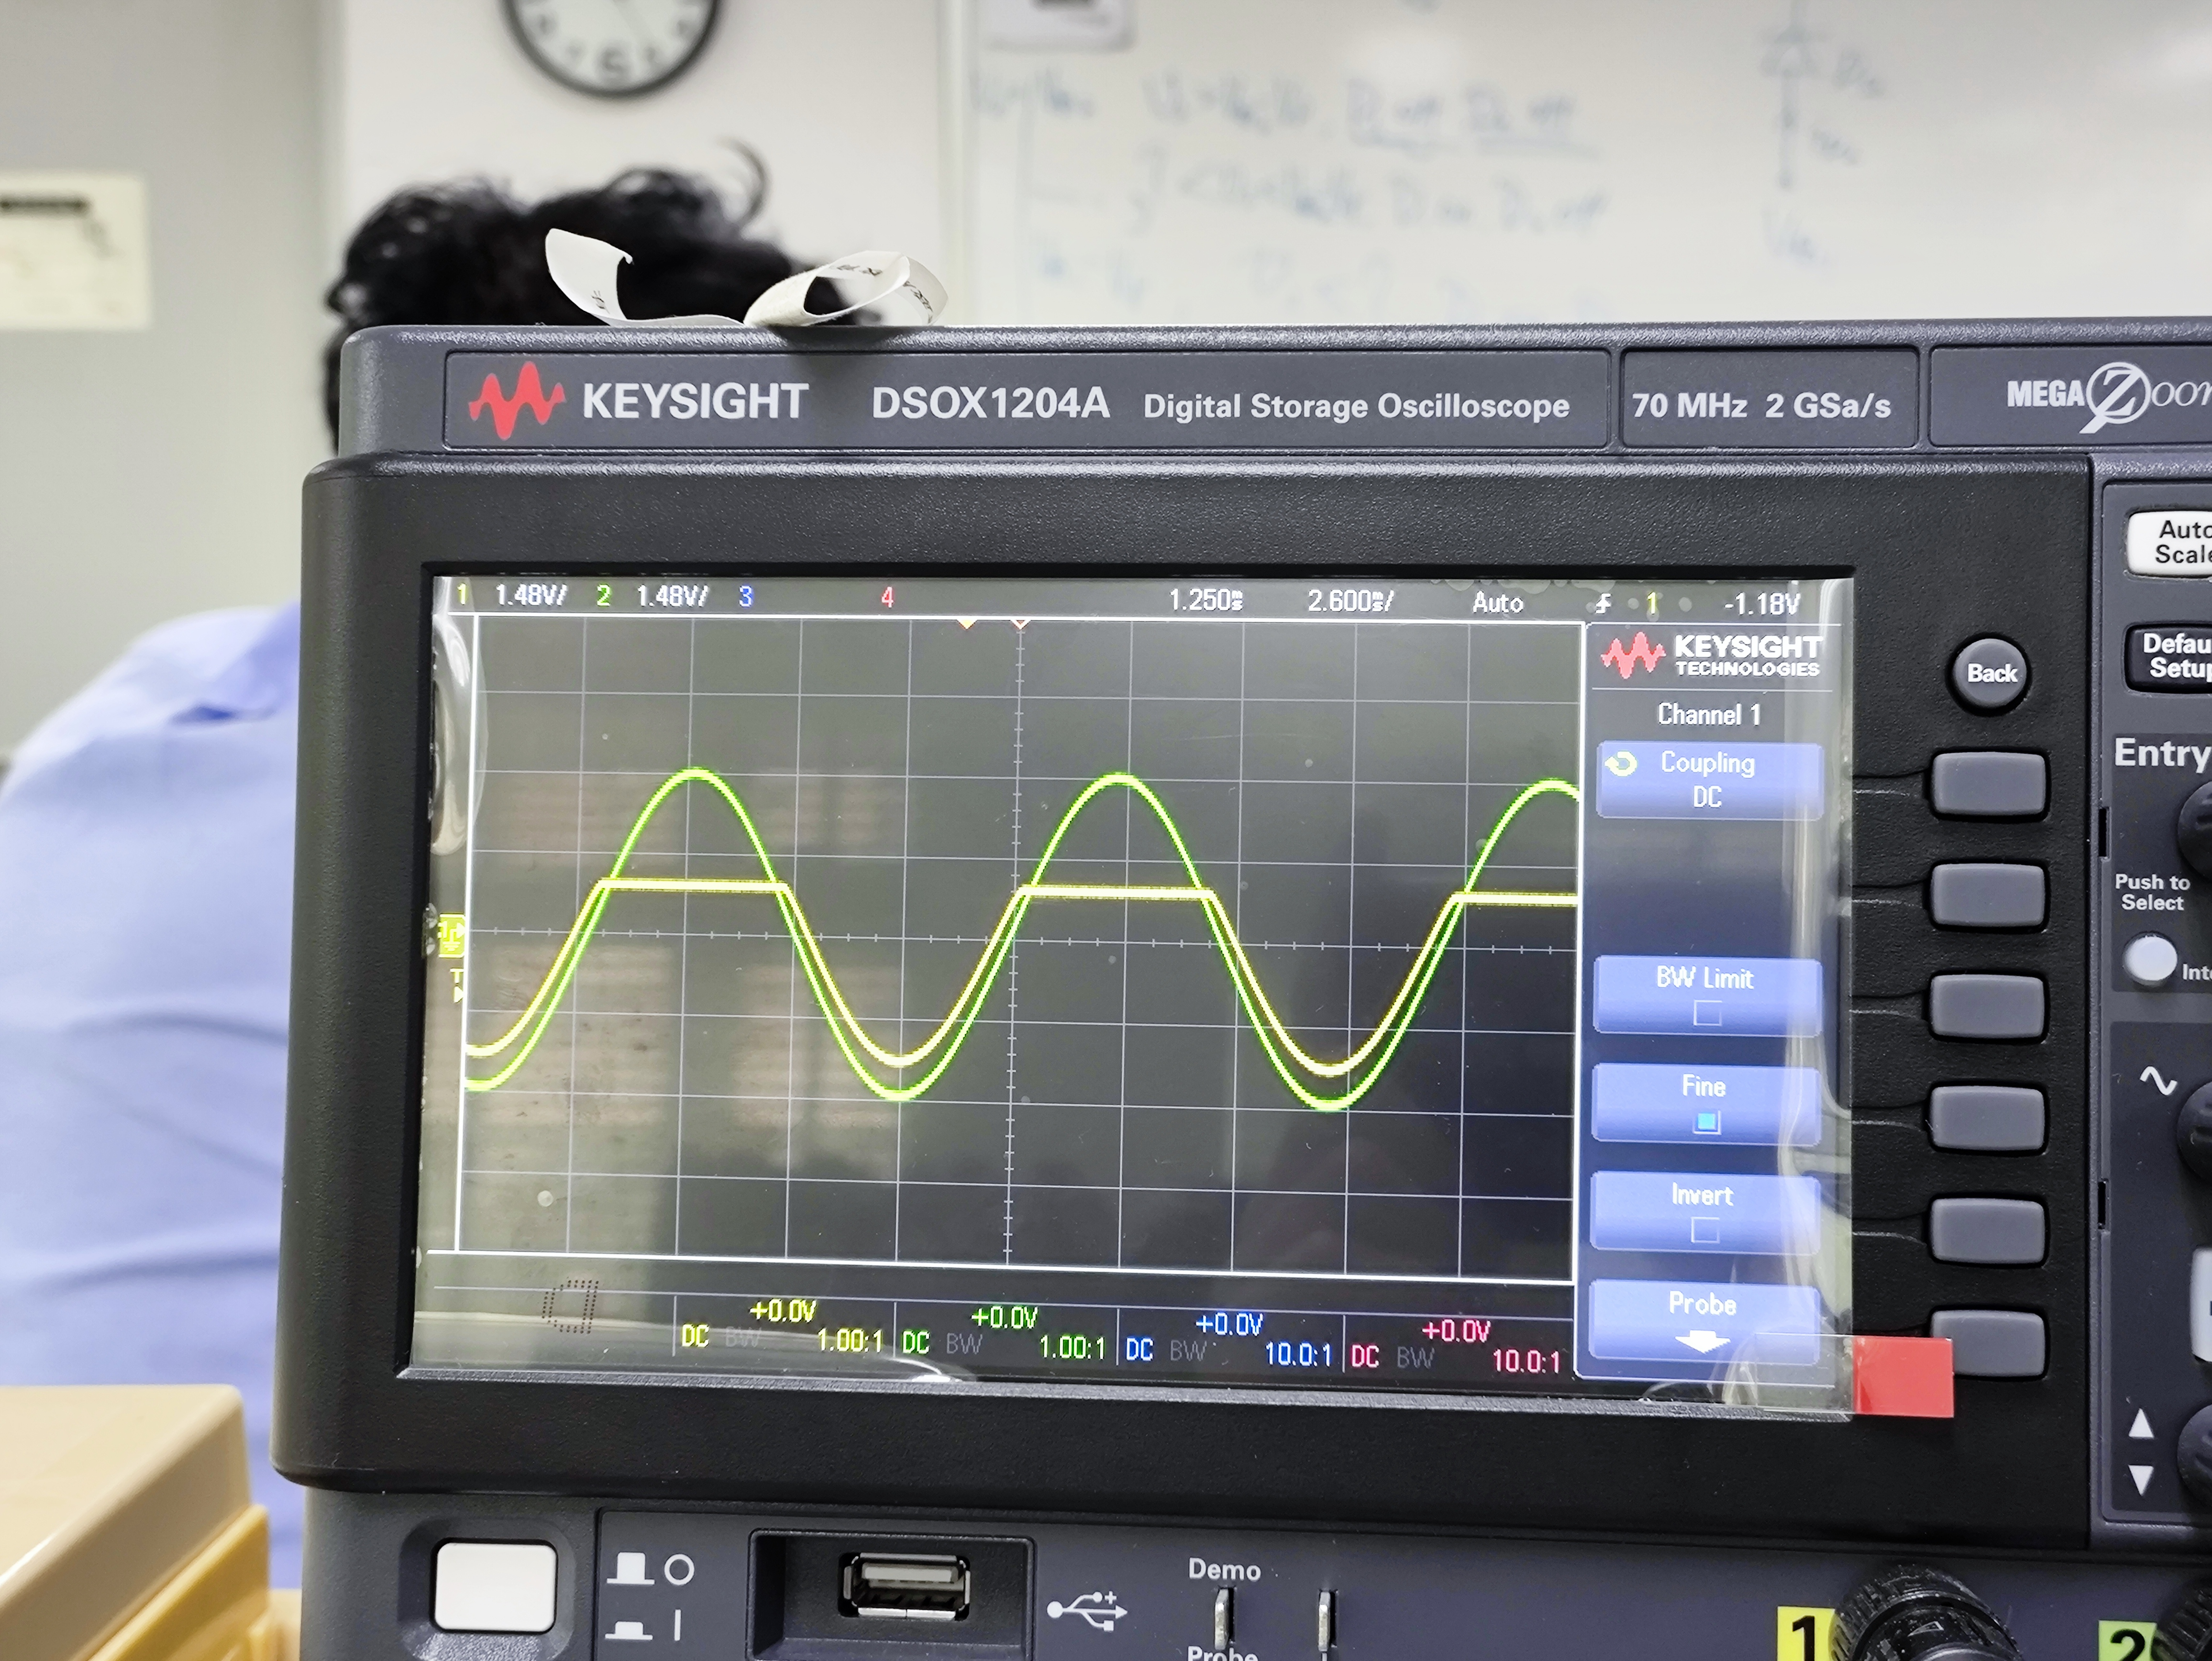
\includegraphics[width=1\linewidth]{Experiment_02/Images/2.5_sin_clipper1.jpg}
                \caption{Sin input signal}
                \label{wave:2bSin}
            \end{subfigure}
            \begin{subfigure}{0.45\textwidth}
                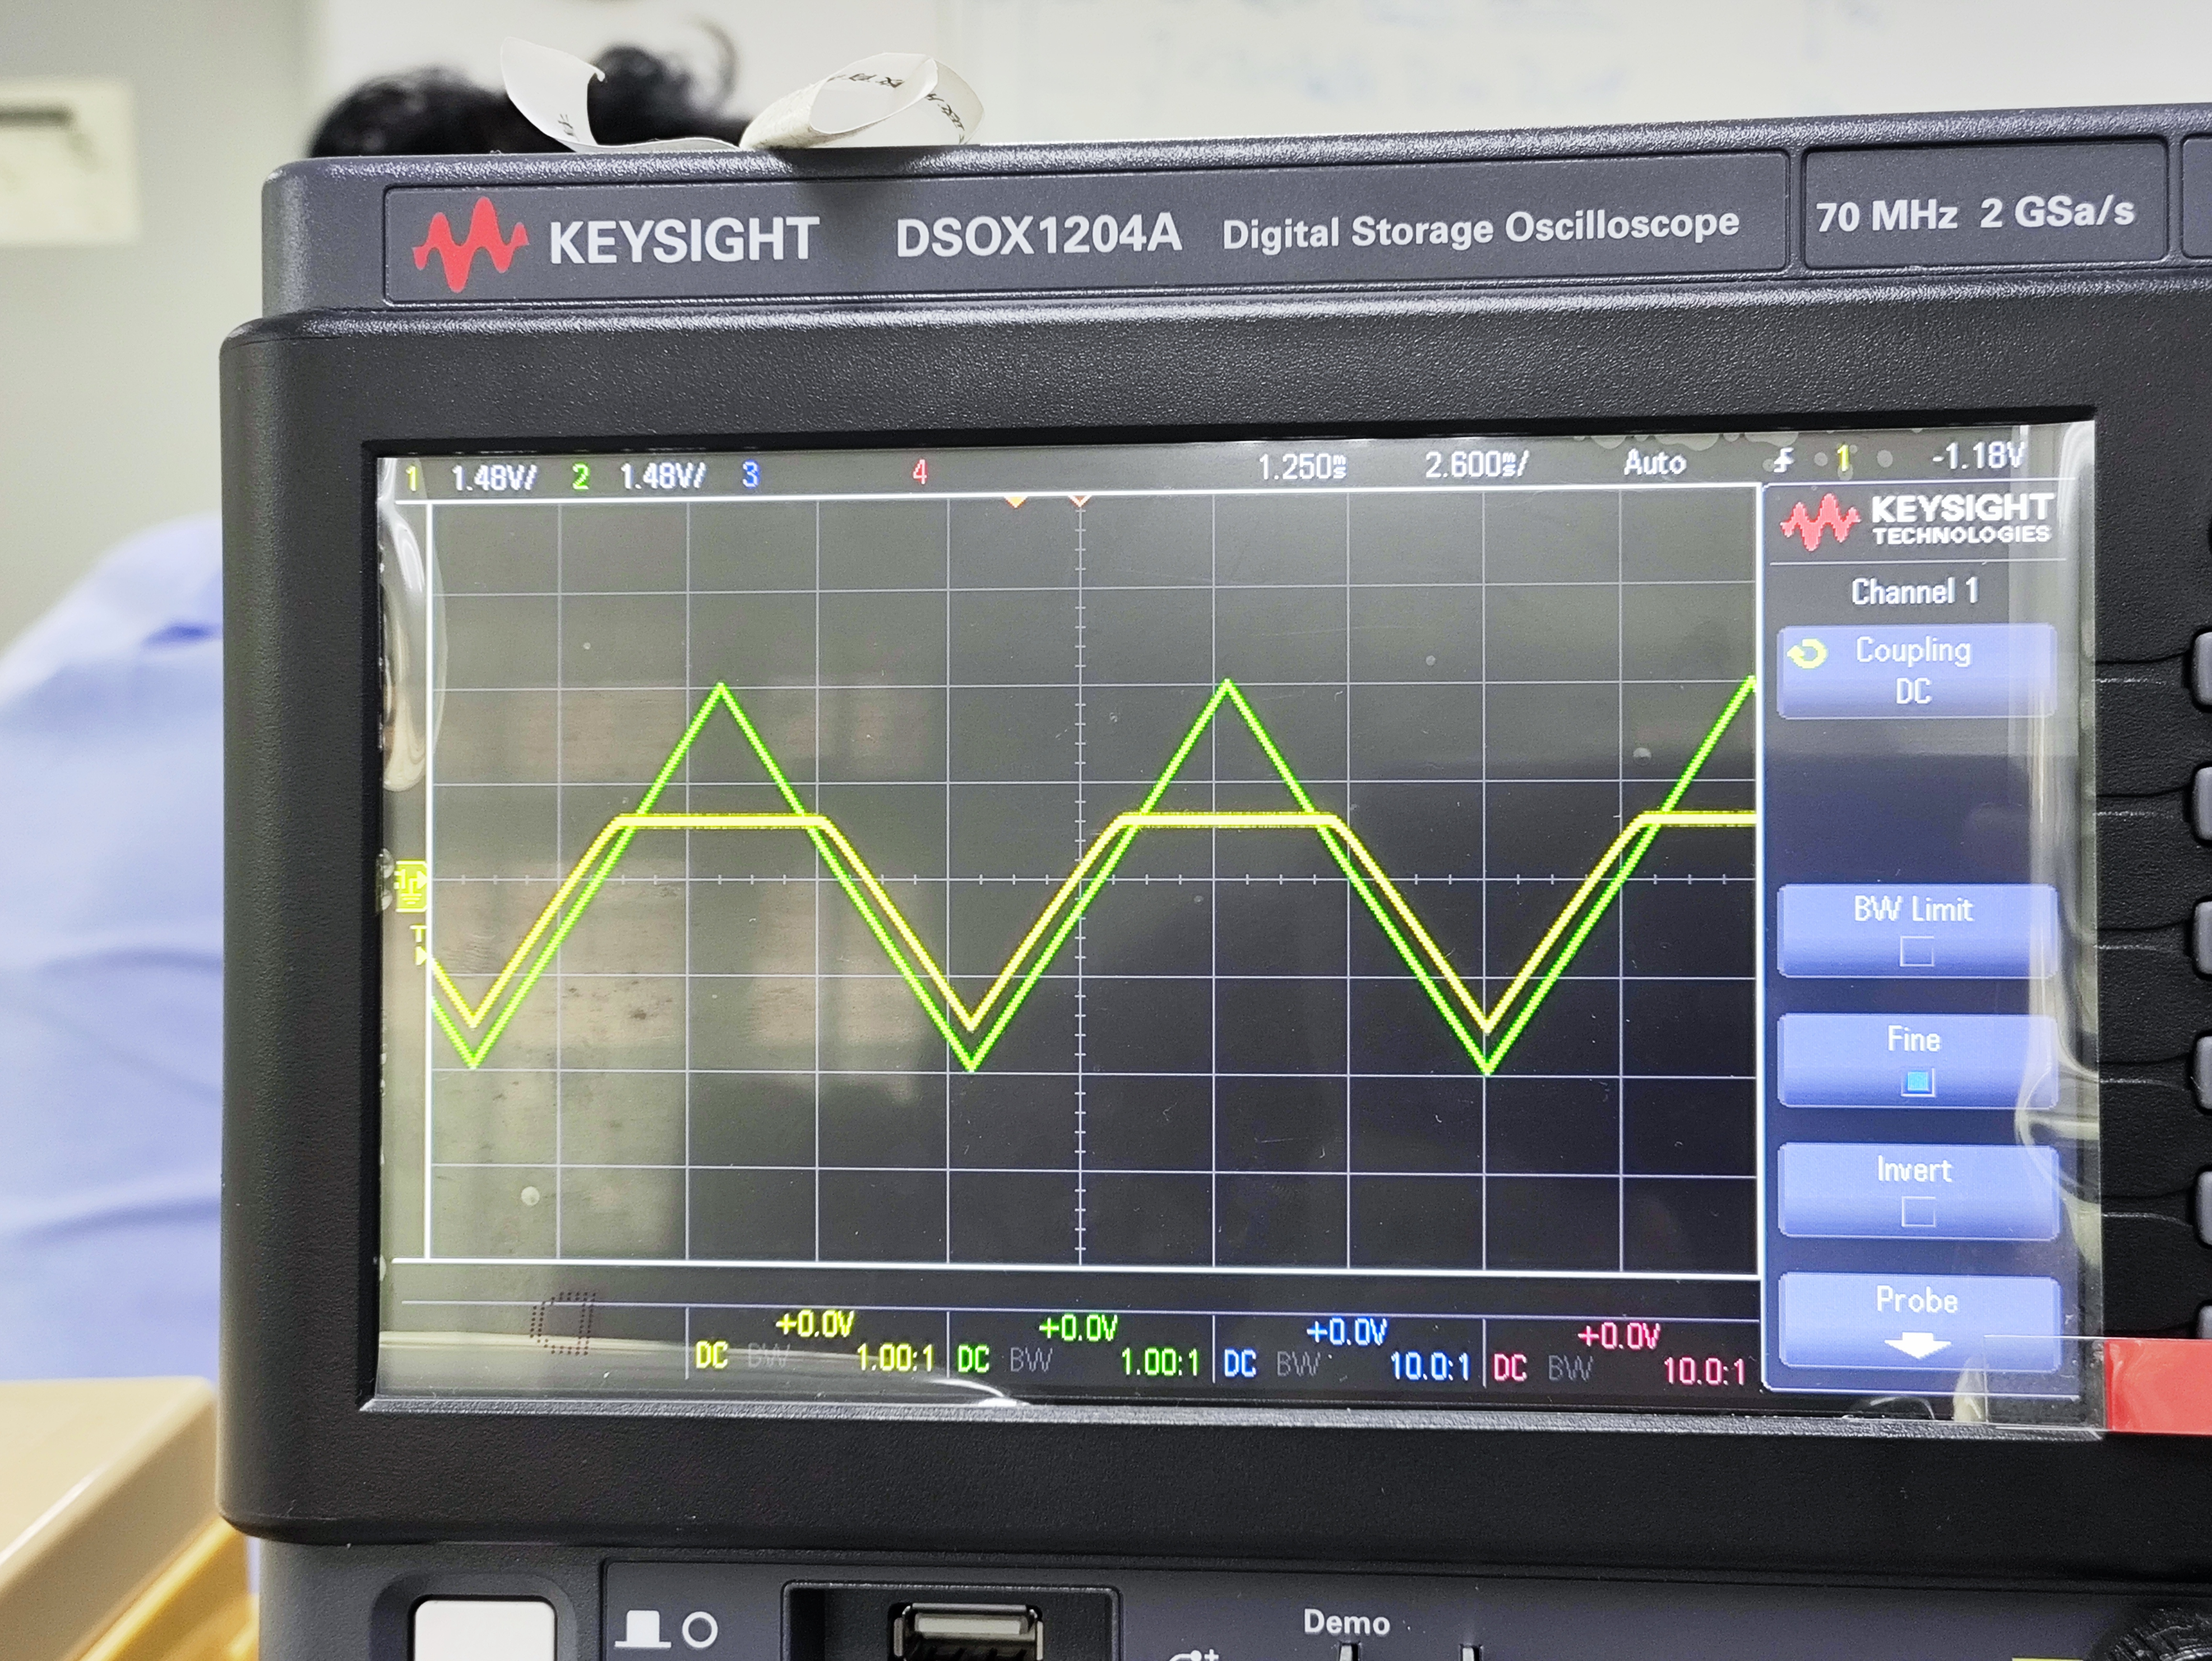
\includegraphics[width=1\linewidth]{Experiment_02/Images/2.5_tri_clipper1.jpg}
                \caption{Triangular input signal}
                \label{wave:2bTri}
            \end{subfigure}
            \caption{The output singal of Clipper circuit}
        \end{figure}
        
        \item \textbf{Data Analysis}\newline
            The theoretical output voltage of the half-wave rectifier is caculated according to equation \ref{eq:2clip}, and was put into the table tab\ref{tab:2clip} for reference.\par

            According to the table, the measured output voltage is consistent with the theoretical output voltage. This means the clipper circuit works as expected.\par

            In the wavefrom plot in fig\ref{wave:2bSin} and fig\ref{wave:2bTri}, we can see the input signal is clipped by the circuit, and only portion of the input is shown in output.\par
    \end{enumerate}

    \subsubsection{Clipper Circuit II}
    \begin{enumerate}[I]
        \item \textbf{Data Recorded}\newline
            The recorded data for the integration operation circuit is shown in the following table \ref{tab:}:
            \begin{table}[h]
                \centering
                \begin{tabular}{l|ccccccc}
                    \toprule
                    Vs   & 0     & 0.5   & 1     & 1.5   & 2     & 2.5   & 3     \\
                    Vo   & 4.548 & 4.585 & 4.827 & 5.073 & 5.321 & 5.569 & 5.817 \\
                    Theo & 4.449 & 4.449 & 4.449 & 4.449 & 4.449 & 4.449 & 4.449 \\
                    \midrule
                    \midrule
                    Vs   & 3.5   & 4     & 4.5   & 5     & 5.5   & 6     & 6.5   \\
                    Vo   & 6.066 & 6.312 & 6.561 & 6.805 & 7.05  & 7.294 & 7.534 \\
                    Theo & 4.449 & 4.865 & 5.319 & 6.364 & 6.818 & 7.273 & 7.727 \\
                    \midrule
                    \midrule
                    Vs   & 7     & 7.5   & 8     & 8.5   & 9     & 9.5   & 10    \\
                    Vo   & 7.765 & 7.966 & 7.994 & 7.994 & 7.994 & 7.994 & 7.994 \\
                    Theo & 7.137 & 8     & 8     & 8     & 8     & 8     & 8     \\
                    \midrule
                \end{tabular}
                    \caption{Recorded Data for half-wave rectifier}
                \label{tab:2clip2}
            \end{table}
        And here are the plot of response with respect to the input signal:
        \begin{figure}[H]
            \centering
            \begin{subfigure}{0.45\textwidth}
                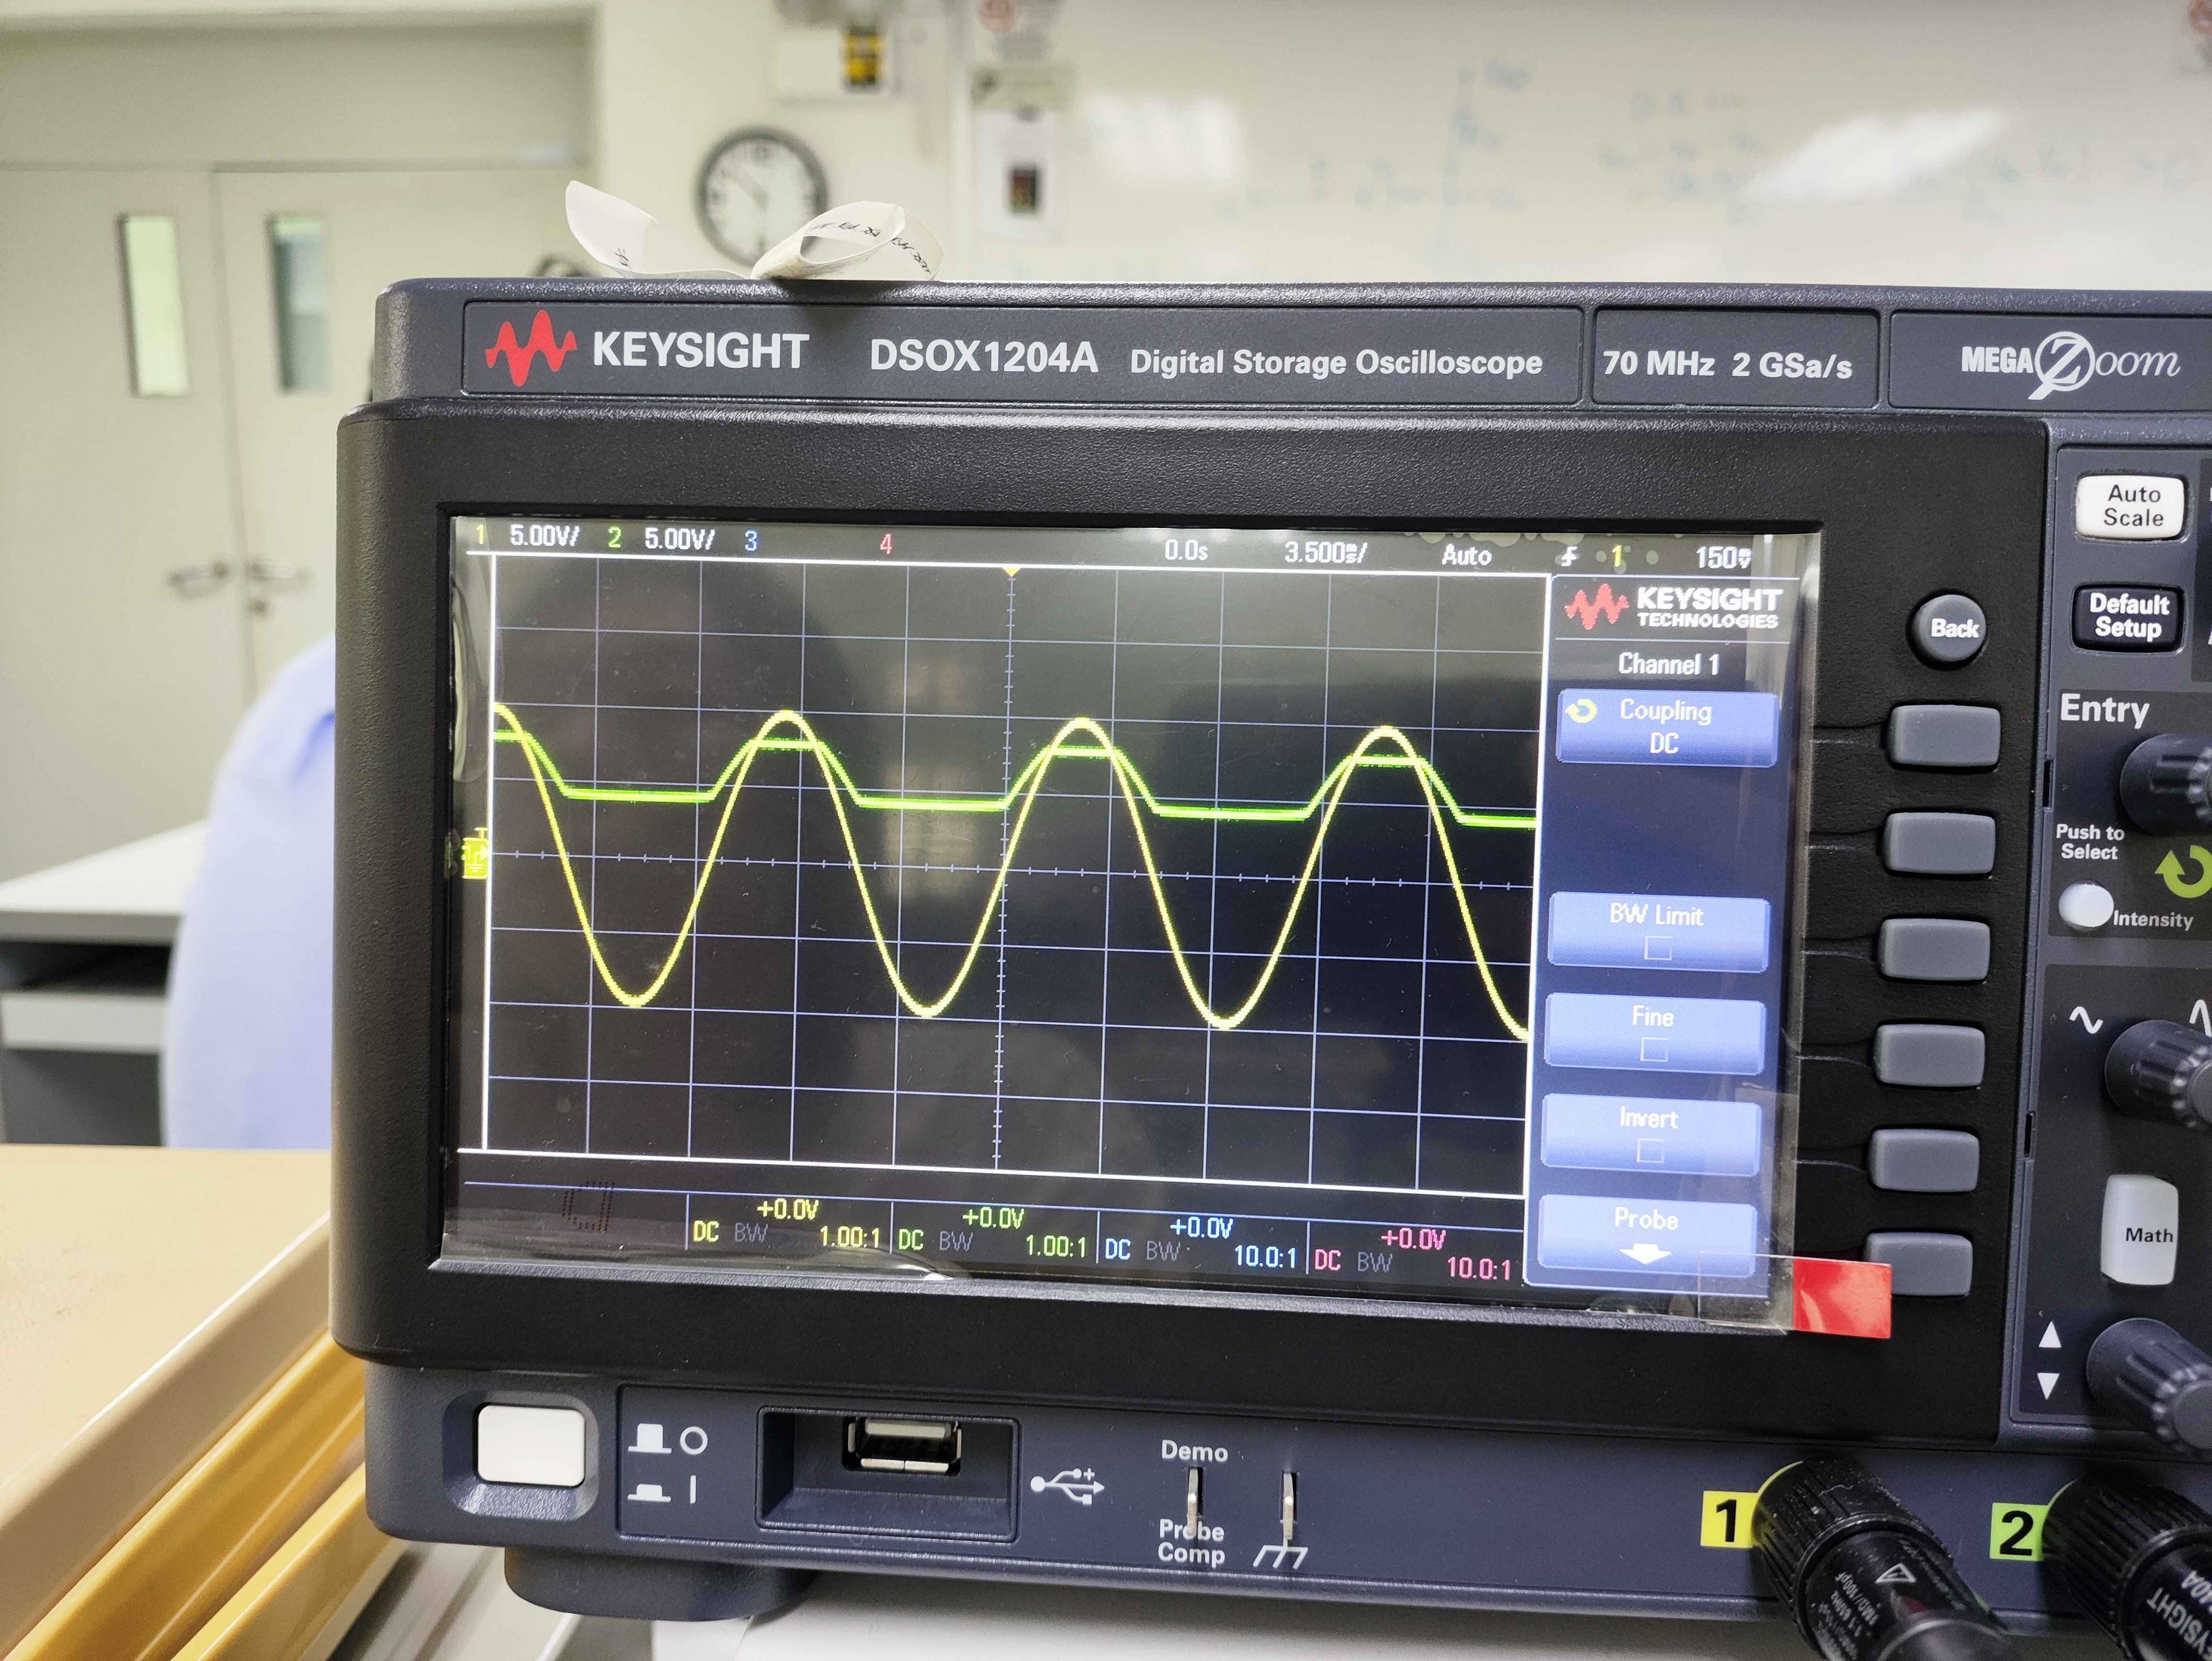
\includegraphics[width=1\linewidth]{Experiment_02/Images/2.6_sin_clipper2.jpg}
                \caption{Sin input signal}
                \label{wave:2cSin}
            \end{subfigure}
            \begin{subfigure}{0.45\textwidth}
                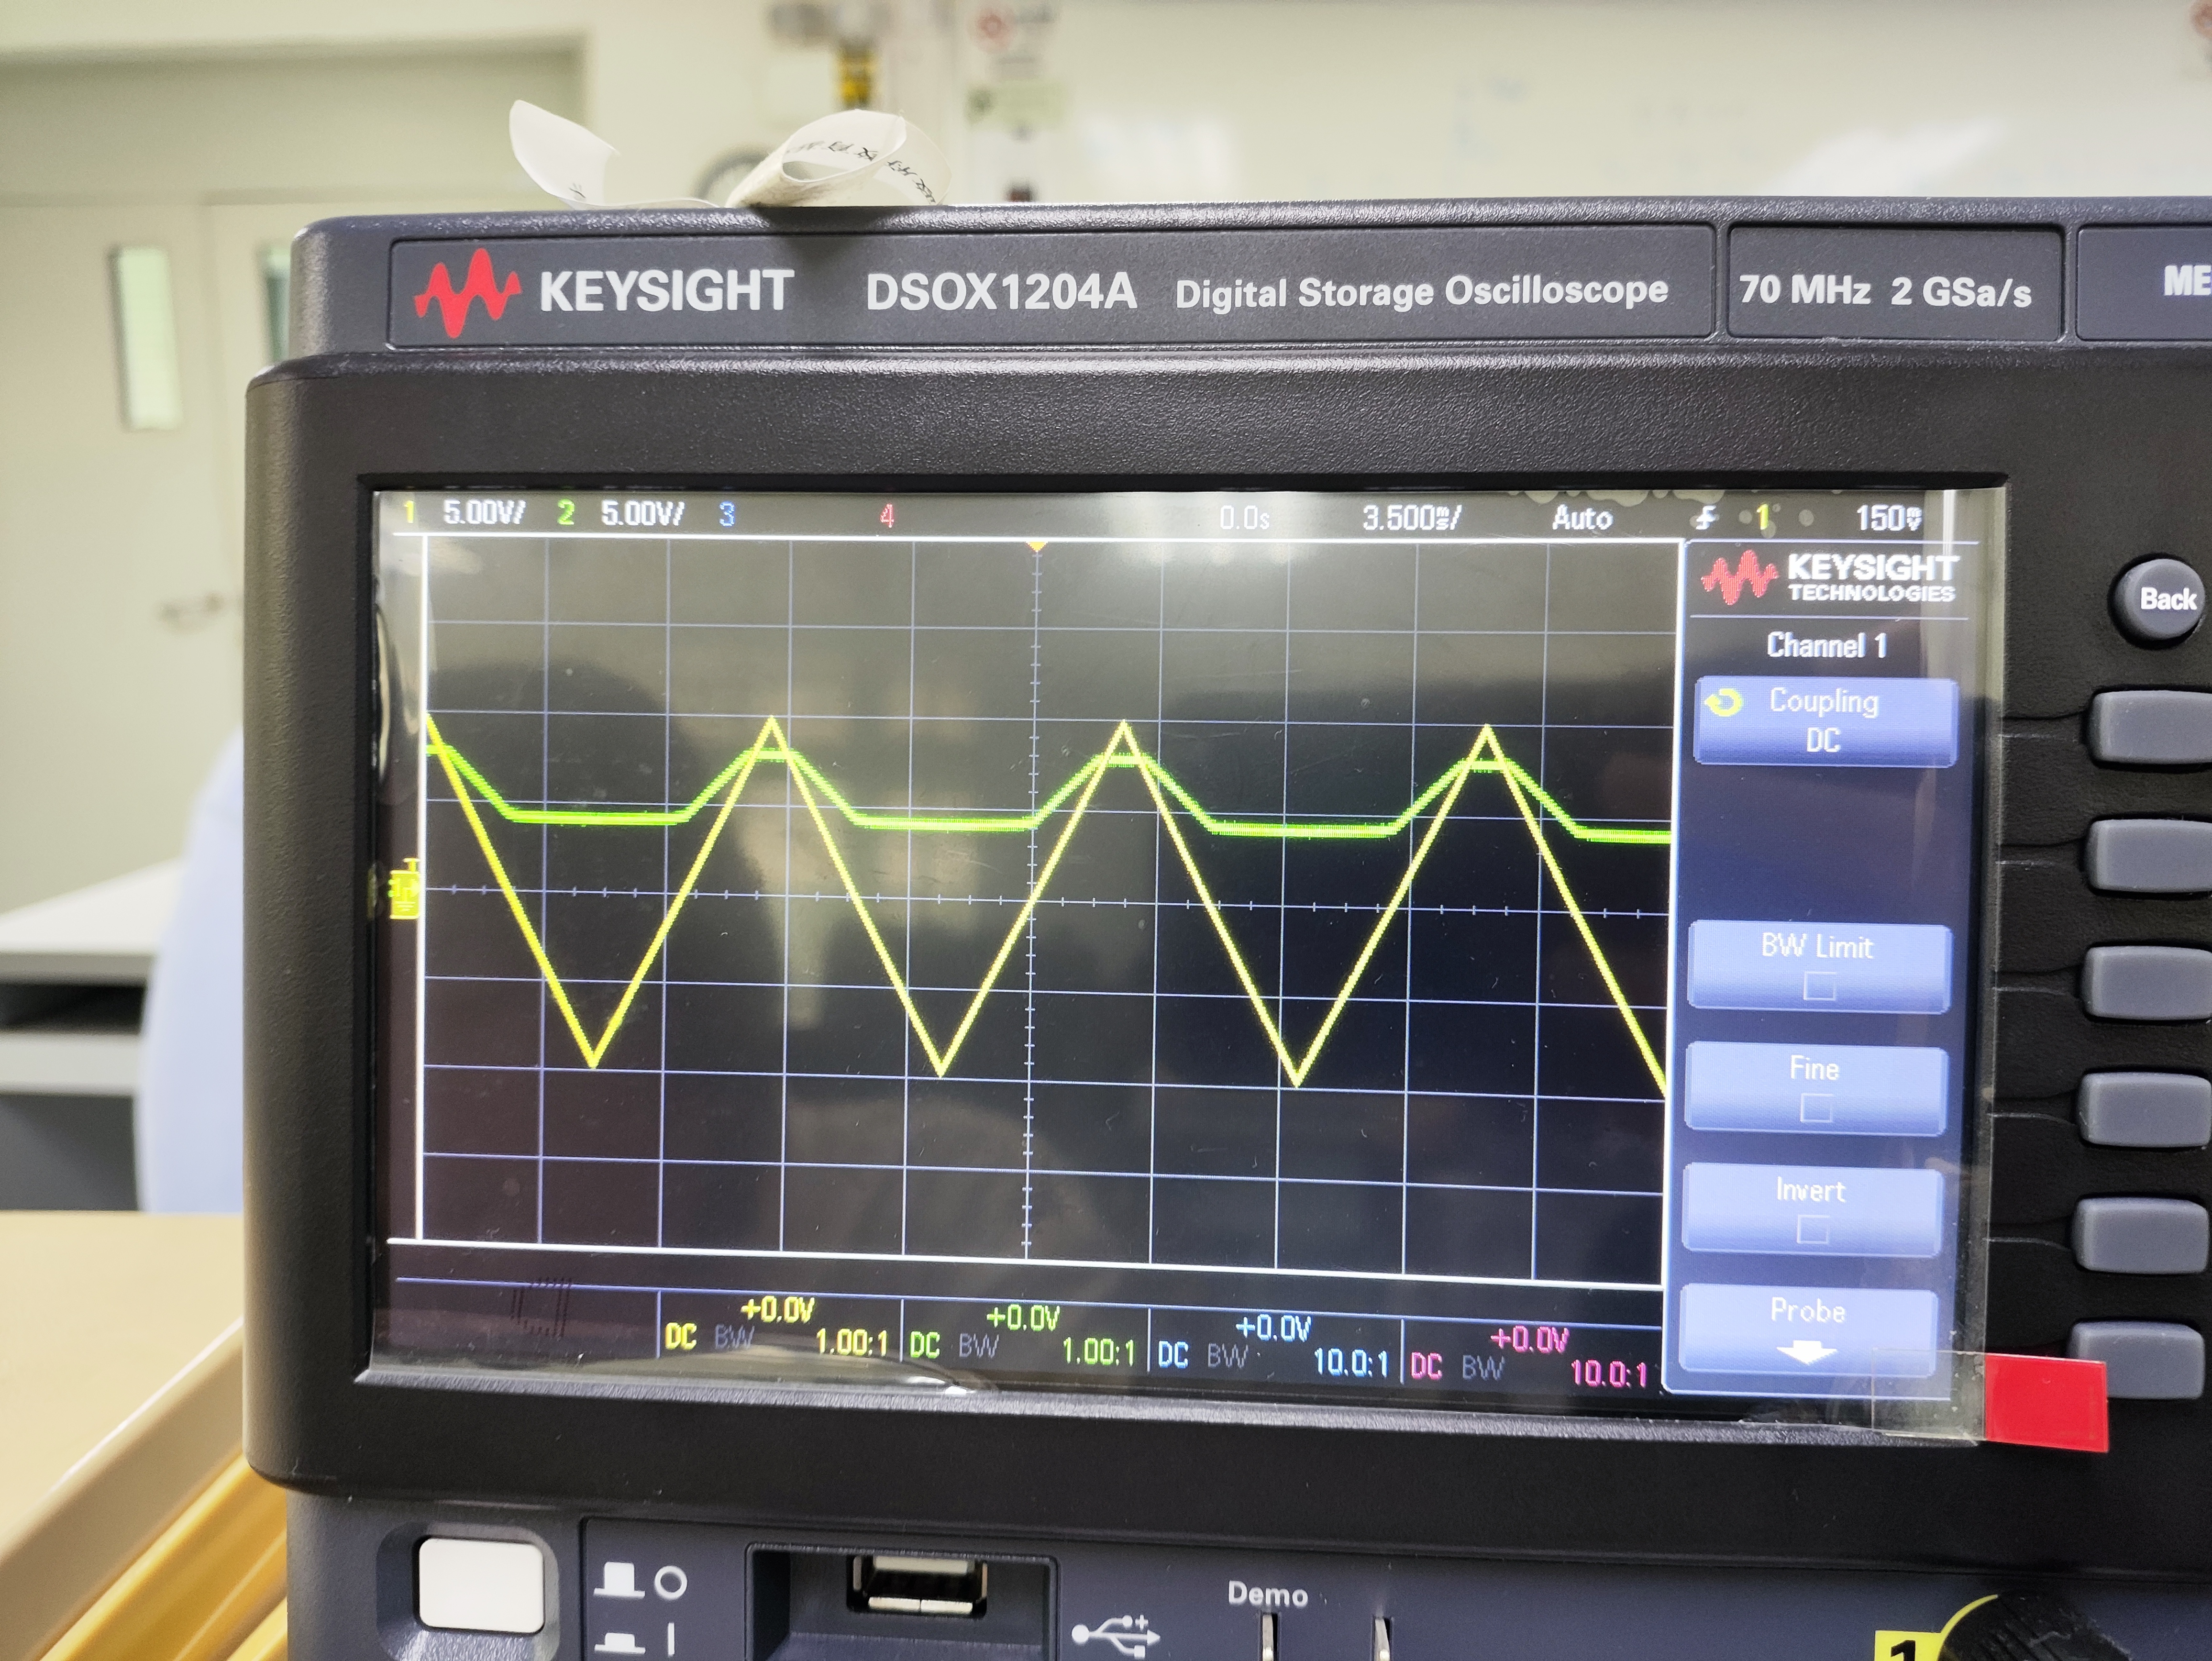
\includegraphics[width=1\linewidth]{Experiment_02/Images/2.6_tri_clipper2.jpg}
                \caption{Triangular input signal}
                \label{wave:2cTri}
            \end{subfigure}
            \caption{The output singal of Clipper circuit II}
        \end{figure}
        
        \item \textbf{Data Analysis}\newline
            The theoretical output voltage of the half-wave rectifier is caculated according to equation \ref{eq:2clip2}, and was put into the table tab\ref{tab:2clip2} for reference.\par

            According to the table, the measured output voltage is consistent with the theoretical output voltage. This means the clipper circuit works as expected.\par

            In the wavefrom plot in fig\ref{wave:2cSin} and fig\ref{wave:2cTri}, we can see the top and bottom of the input signal is clipped by the circuit, and only portion of the input is shown in output.\par
    \end{enumerate}

    \subsubsection{Clamper Circuit}
    \begin{enumerate}[I]
        \item \textbf{Data Recorded}\newline
            The recorded plot of response with respect to the input signal:
        \begin{figure}[H]
            \centering
            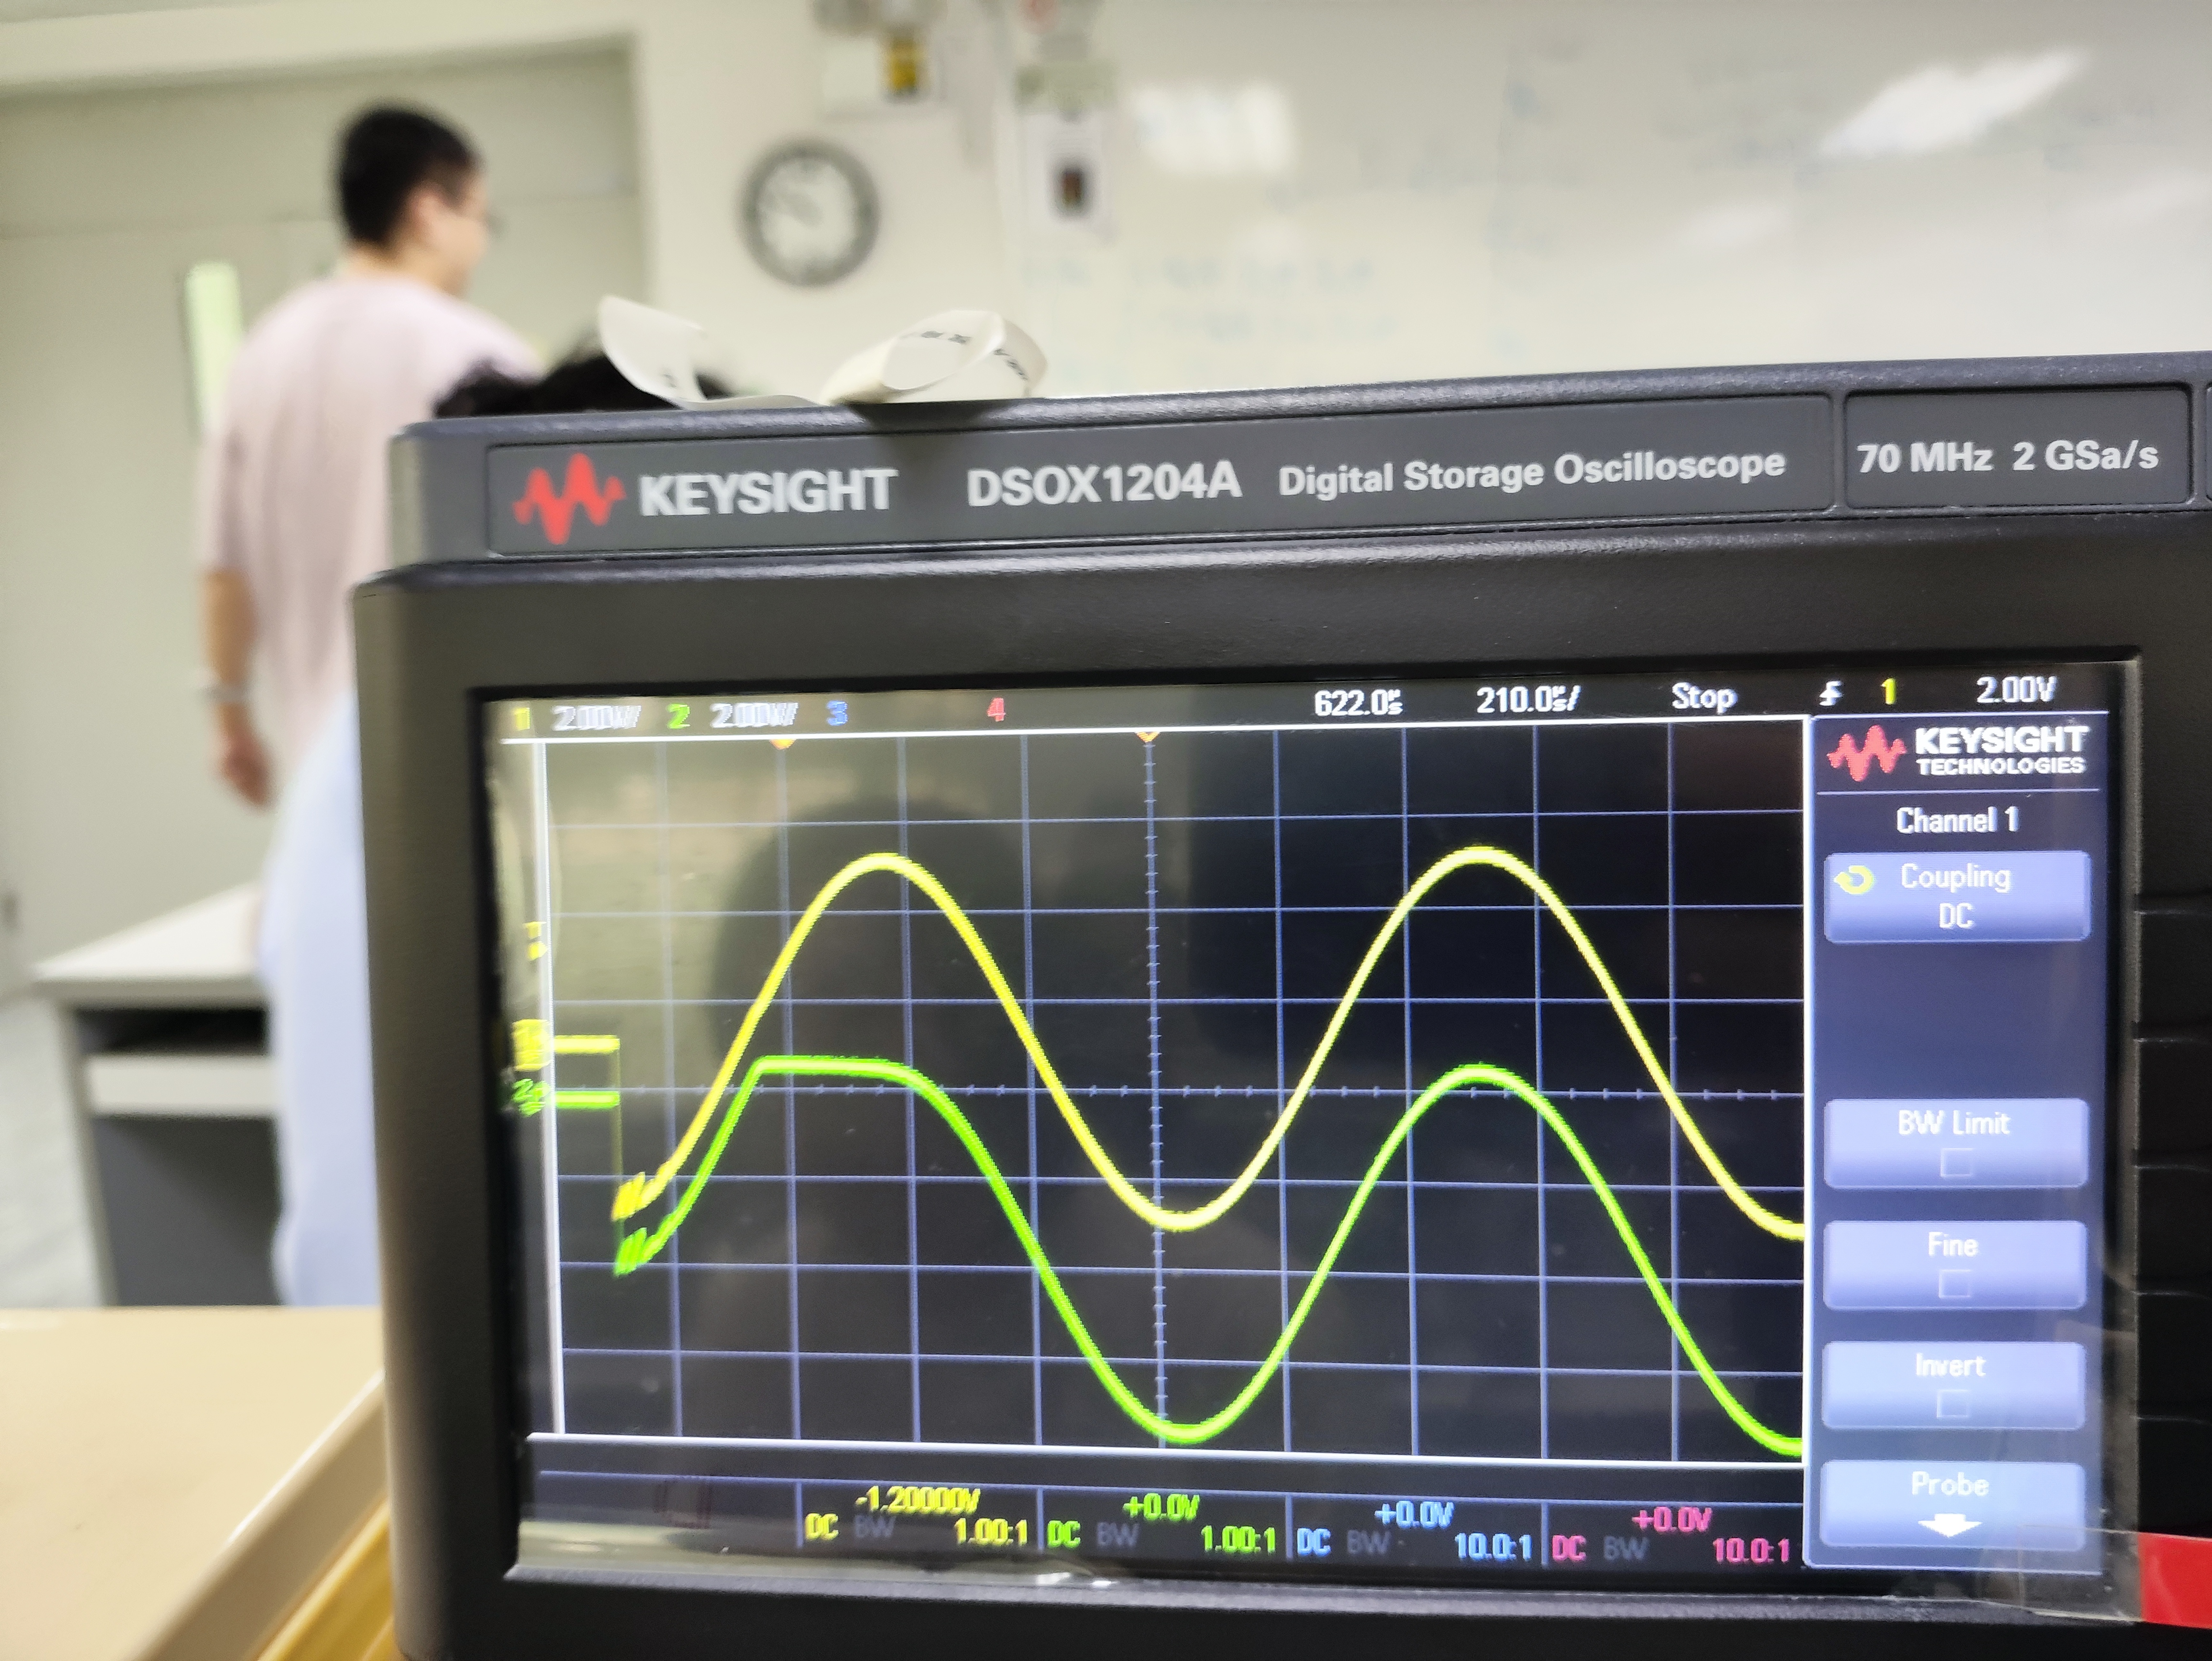
\includegraphics[width=0.5\linewidth]{Experiment_02/Images/2.7_sin_clamper.jpg}
            \caption{The output singal of Clamper circuit}
            \label{wave:2dSin}
        \end{figure}
        
        \item \textbf{Data Analysis}\newline
            In the wavefrom plot in fig\ref{wave:2dSin}, we can see the output signal is shit downward in the y axis. This is beacuse the capacitor will be charge when the input signal is positive, and slowly discharge when the input signal is negetive.\par
    \end{enumerate}
    
\subsection{Experiment Conclusion}
    \subsubsection{Conclusion}
    In this experiment, we constructed three types of diode circuit, and tested their behaviour using the DMM and Oscilloscope. Finally, we conclude our calculation is correct.